\documentclass{article}
\usepackage{graphicx}
\usepackage{titling}  % For custom title page
\usepackage{circuitikz}
\usepackage{matlab-prettifier}
\usepackage{amsmath}
\usepackage{amssymb}
\usepackage{booktabs,tabu}
\usepackage[section]{placeins}


\title{Experiment 1: Basic Filter Design}
\author{Samyak Sheersh}
\date{13 August 2024}
\newcommand{\subtitle}[1]{%
  \posttitle{%
    \par\end{center}
    \begin{center}\large#1\end{center}
    \vskip0.5em}%
}

\begin{document}

% Custom title page
\begin{titlepage}
    \centering
    
\includegraphics[width=0.2\textwidth]{KGP_logo.png}\par\vspace{1cm}
    {\scshape\LARGE Department of Electronics and Electrical Communication Engineering, IIT Kharagpur\par}
    \vspace{1cm}
    {\huge\bfseries Experiment 1: Sampling\par}
    \vspace{1.5cm}
    {\Large\itshape Samyak Sheersh, Anubhav Mitra\par}
    \vfill
    % Identifying information at the bottom
    {\large Roll Numbers: 22EC30045, 22EC30007\par}
    {\large Group Number: 24\par}
    \vfill
    {\large 13 August 2024\par}
\end{titlepage}

\section{Objectives}
\begin{enumerate}
  \item To design FIR filters for various orders and cutoff frequencies.
  \item To assess whether passband and stop band frequencies are attenuated by the filter designed.
  \item To assess the response of such FIR filters to noise contaminated signals. 
\end{enumerate}

\section{Definitions of windows and LPF}

\subsection{LPF}
\begin{equation}
  h_d[n] = \begin{cases} \frac{\omega_c}{\pi} & n=k  \\ \frac{\sin(\omega_c (n-k))}{\pi(n-k)} & otherwise \end{cases}
\end{equation}



\subsection{Rectangular Window}
\begin{equation}
  w[n] = \begin{cases}  1 & n=0,1,\dots, N-1  \\ 0 & otherwise \end{cases}
\end{equation}

\subsection{Triangular Window}
\begin{equation}
  w[n] = \begin{cases}  1-2 \frac{n-\frac{N-1}{2}}{N-1} & n=0,1,\dots, N-1  \\ 0 & otherwise \end{cases}
\end{equation}

\subsection{Hanning Window}
\begin{equation}
  w[n] = \begin{cases}  \frac{1}{2}-\frac{1}{2} \cos(\frac{2\pi n}{N-1}) & n=0,1,\dots, N-1  \\ 0 & otherwise \end{cases}
\end{equation}

\subsection{Hanning Window}
\begin{equation}
  w[n] = \begin{cases}  0.54-0.46 \cos(\frac{2\pi n}{N-1}) & n=0,1,\dots, N-1  \\ 0 & otherwise \end{cases}
\end{equation}

\subsection{Blackmann Window}
\begin{equation}
  w[n] = \begin{cases}  0.42-0.5 \cos(\frac{2\pi n}{N-1}) + 0.08 \cos(\frac{4\pi n}{N-1}) & n=0,1,\dots, N-1  \\ 0 & otherwise \end{cases}
\end{equation}


\section{Observation Tables, Graphs and Diagrams}
\subsection{Rectangular Window}
\begin{center}
\begin{tabular}{||c c c c||} 
 \hline
 N & Transition Width (kHz) & First Side Lobe (dB) & Max Attenuation (dB)\\ [0.5ex] 
 \hline\hline
 8 & 2.30 & -19.4 & -45 \\ 
 64 & 0.25 & -20.9 & -51 \\
 512 & 0.02 & -21.1 & -70 \\   
 \hline
\end{tabular}
\end{center}
Outputs of the \texttt{freqz} function
  \subsubsection{N=8}
  \begin{figure}[!htb]
  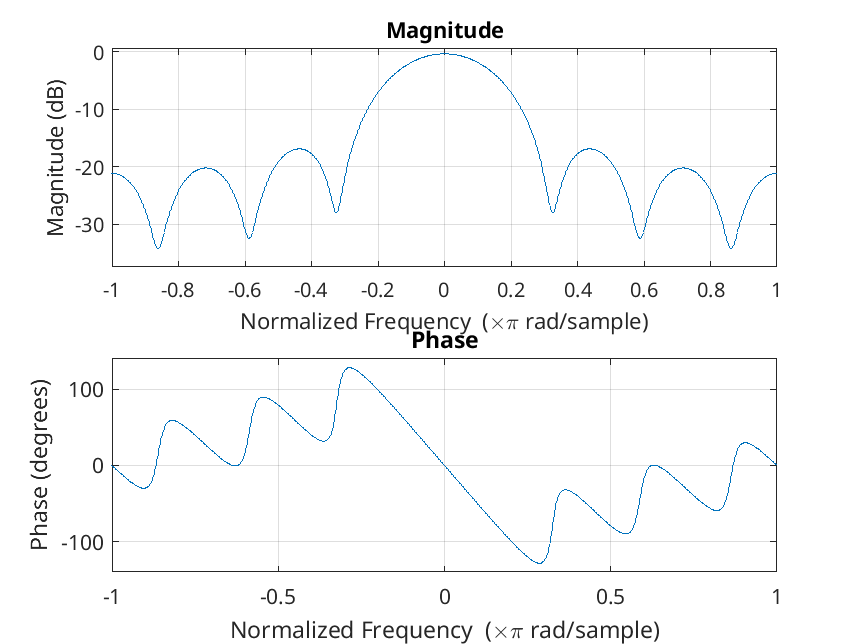
\includegraphics[width=10cm]{freqz_rect_8.png}
  \end{figure}
  \subsubsection{N=64}
  \begin{figure}[!htb]
  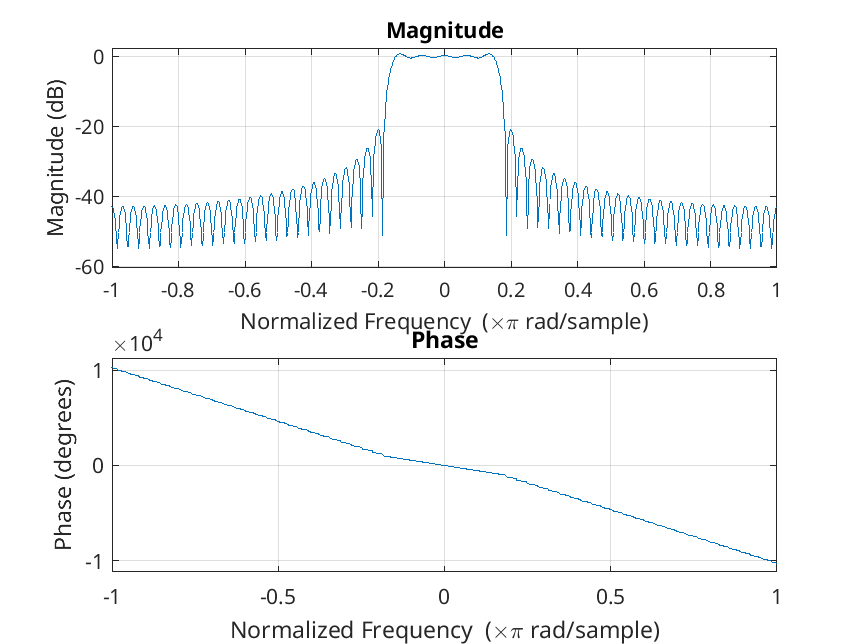
\includegraphics[width=10cm]{freqz_rect_64.png}
  \end{figure}
  \subsubsection{N=512}
  \begin{figure}[!htb]
  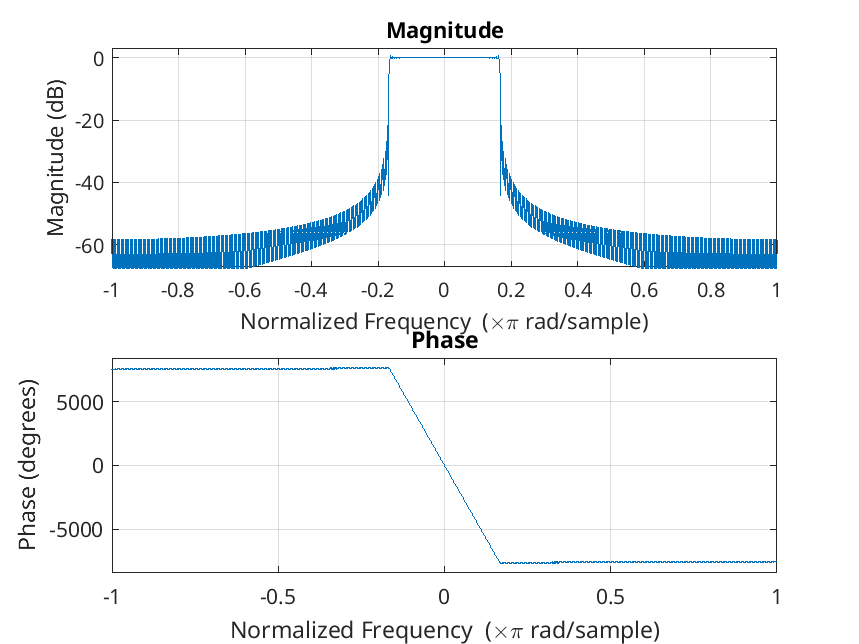
\includegraphics[width=10cm]{freqz_rect_512.png}
  \end{figure}
\subsection{Triangular Window}
\begin{center}
\begin{tabular}{||c c c c||} 
 \hline
 N & Transition Width (kHz) & First Side Lobe (dB) & Max Attenuation (dB)\\ [0.5ex] 
 \hline\hline
 8 & 2.63 & -20.9 & -26 \\ 
 64 & 0.28 & -20.6 & -37 \\
 512 & 0.05 & -20.7 & -60 \\   
 \hline
\end{tabular}
\end{center}

  \subsubsection{N=8}
  \begin{figure}[!htb]
  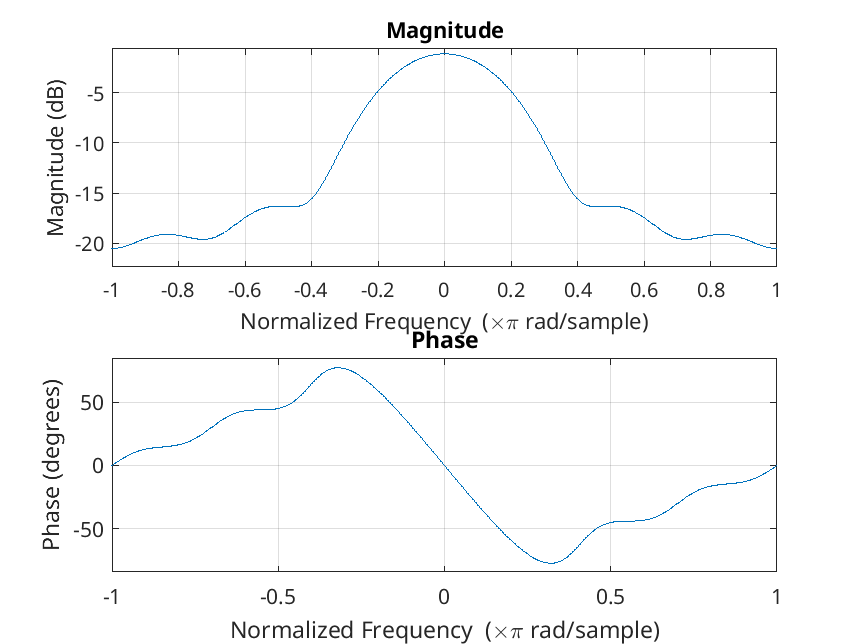
\includegraphics[width=10cm]{freqz_tri_8.png}
  \end{figure}
  \subsubsection{N=64}
  \begin{figure}[!htb]
  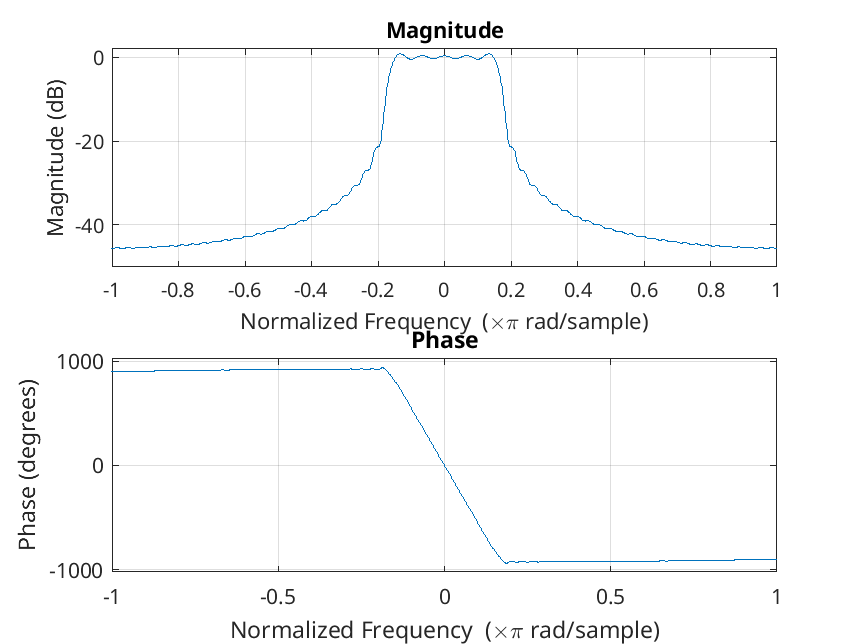
\includegraphics[width=10cm]{freqz_tri_64.png}
  \end{figure}
  \subsubsection{N=512}
  \begin{figure}[!htb]
  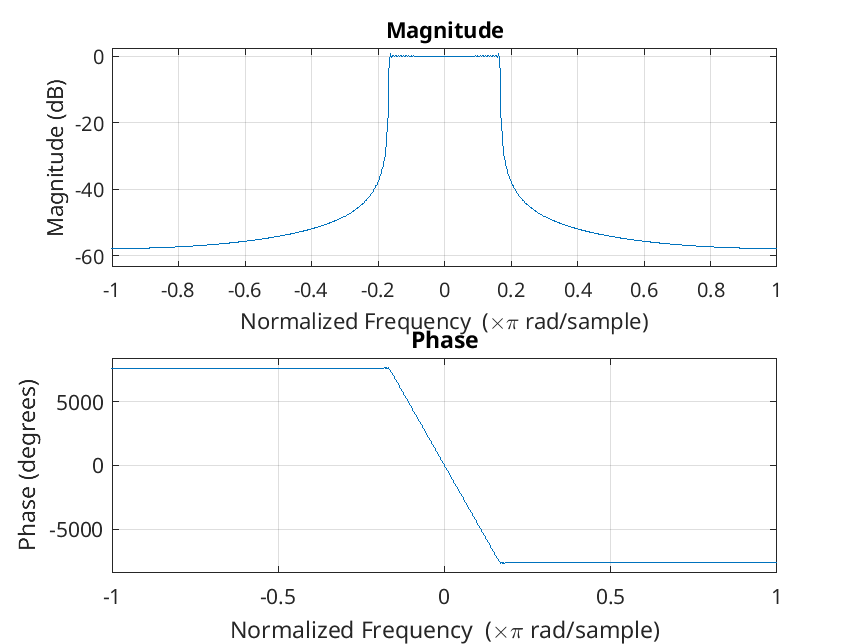
\includegraphics[width=10cm]{freqz_tri_512.png}
  \end{figure} 
\subsection{Hanning Window}
  \subsubsection{N=8}
  \begin{figure}[!htb]
  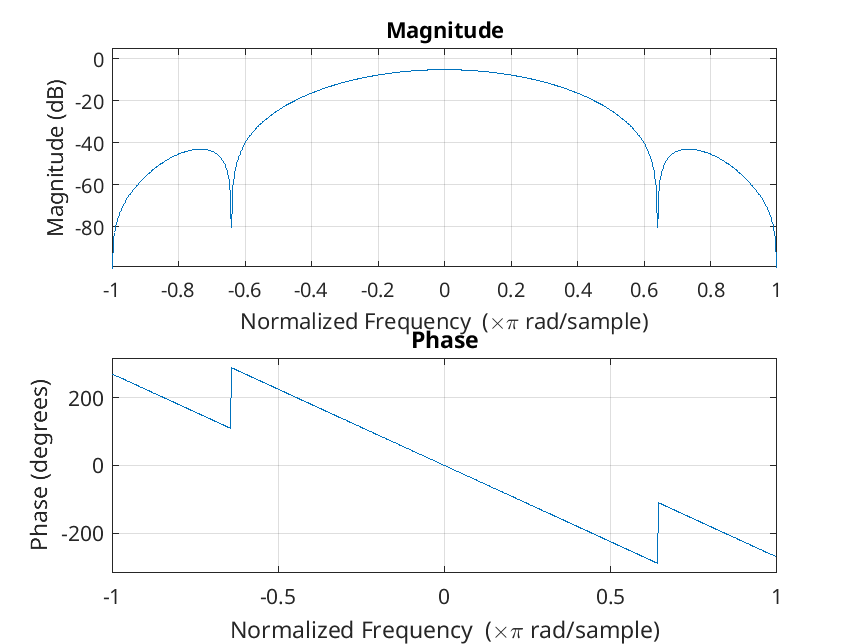
\includegraphics[width=10cm]{freqz_han_8.png}
  \end{figure}
  \subsubsection{N=64}
  \begin{figure}[!htb]
  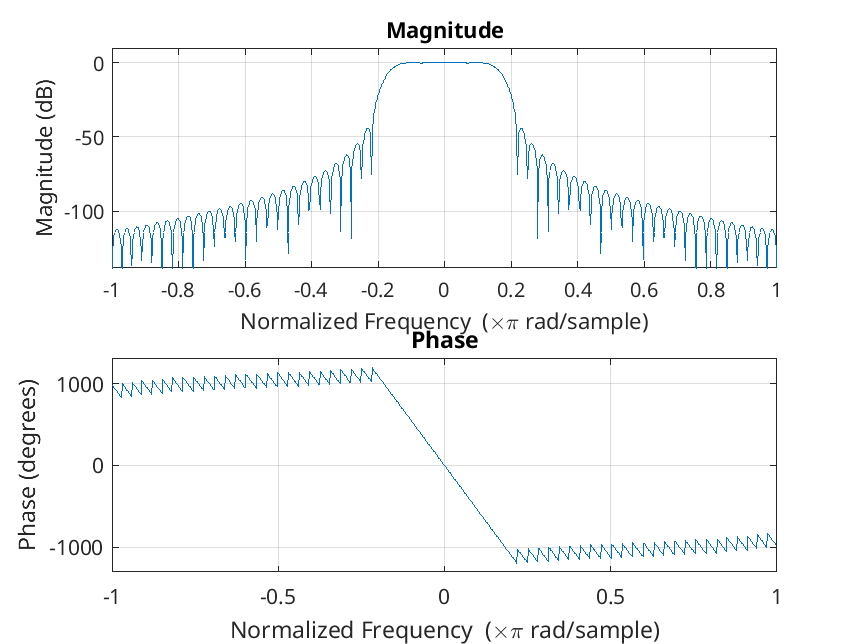
\includegraphics[width=10cm]{freqz_han_64.png}
  \end{figure}
  \subsubsection{N=512}
  \begin{figure}[!htb]
  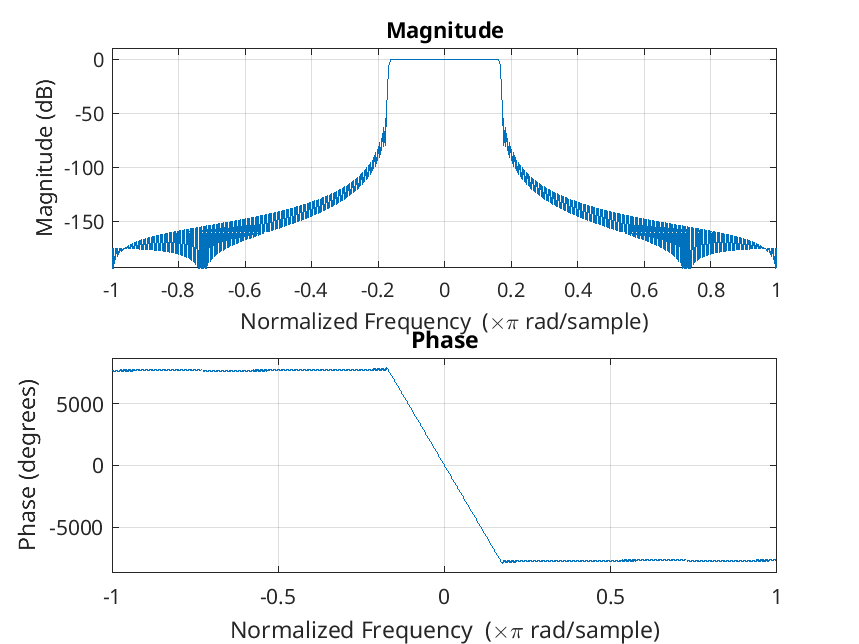
\includegraphics[width=10cm]{freqz_han_512.png}
  \end{figure}
\subsection{Hamming Window}
  \subsubsection{N=8}
  \begin{figure}[!htb]
  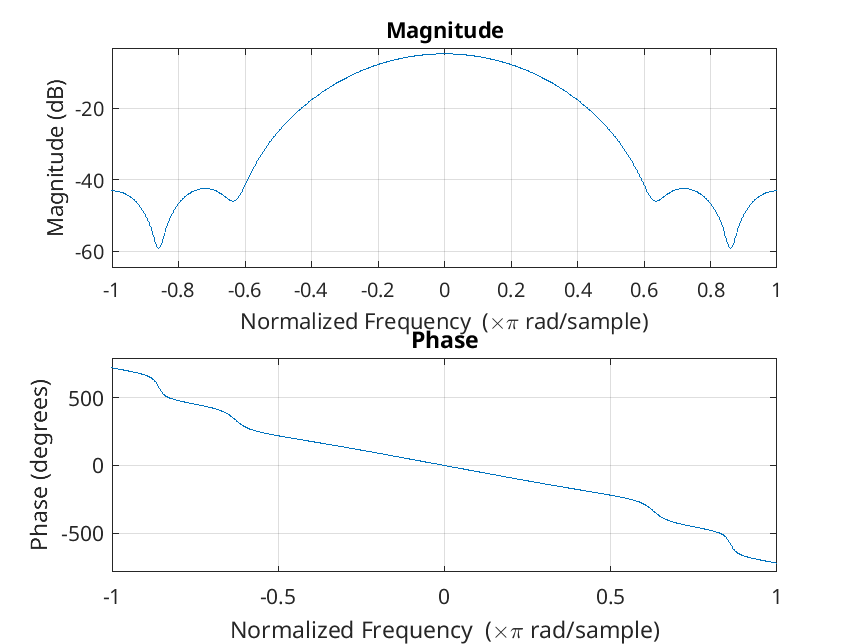
\includegraphics[width=10cm]{freqz_ham_8.png}
  \end{figure}

  \subsubsection{N=64}
  \begin{figure}[!htb]
  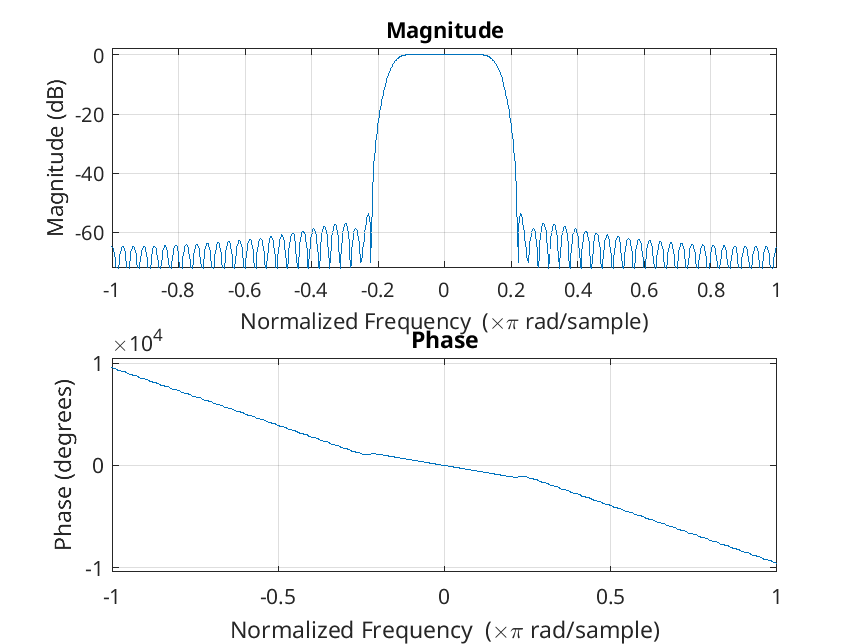
\includegraphics[width=10cm]{freqz_ham_64.png}
  \end{figure}

  \subsubsection{N=512}
  \begin{figure}[!htb]
  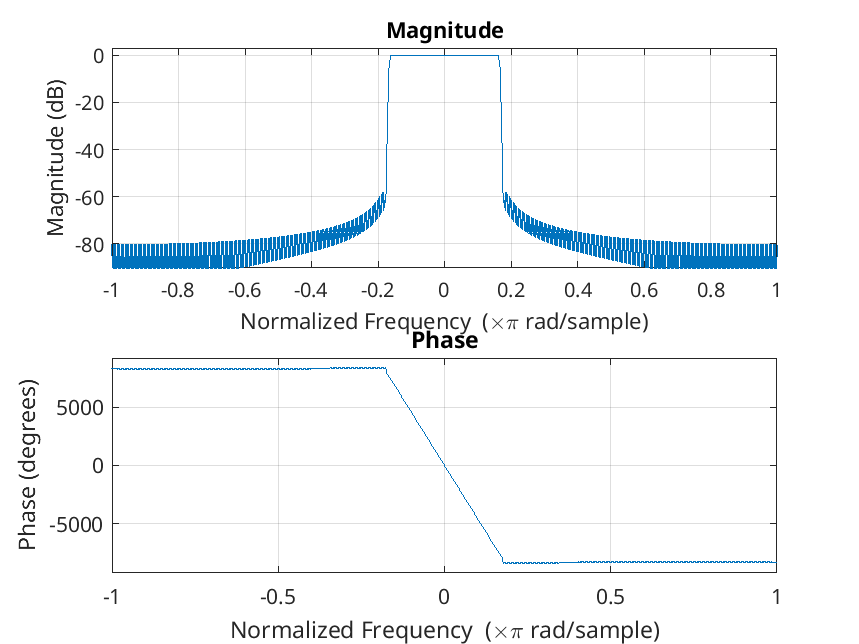
\includegraphics[width=10cm]{freqz_ham_512.png}
  \end{figure}

\subsection{Blackmann Window}
  \subsubsection{N=8}
  \begin{figure}[!htb]
  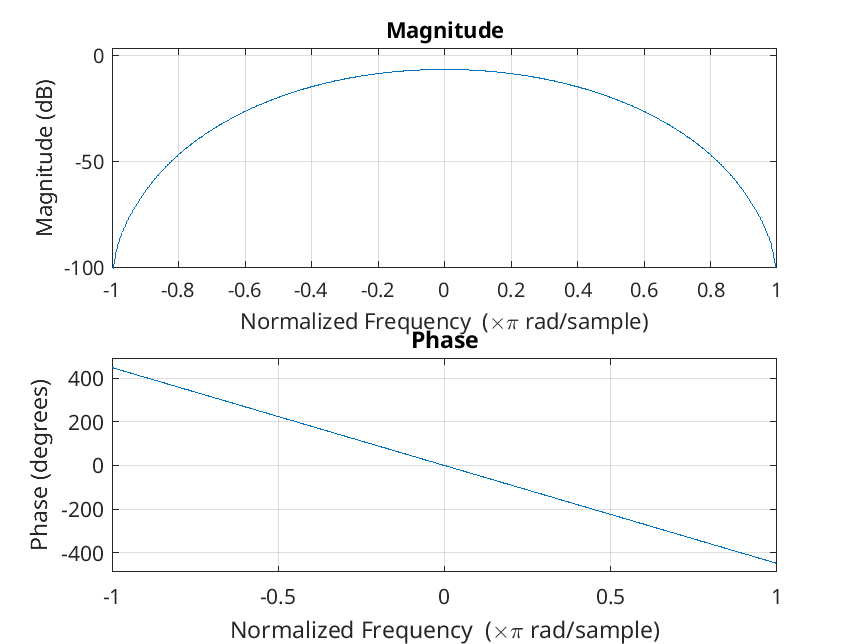
\includegraphics[width=10cm]{freqz_bl_8.png}
  \end{figure}

  \subsubsection{N=64}
  \begin{figure}[!htb]
  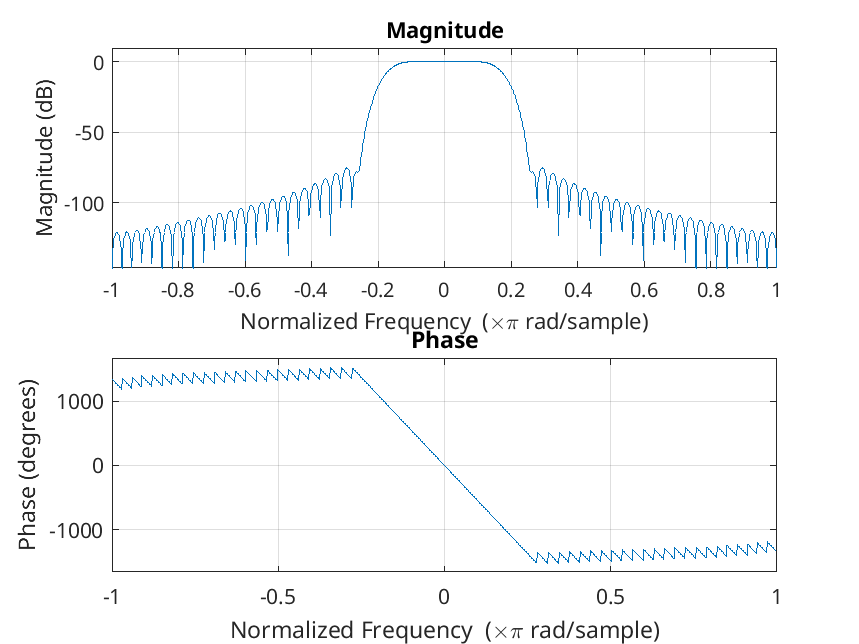
\includegraphics[width=10cm]{freqz_bl_64.png}
  \end{figure}
  \subsubsection{N=512}
  \begin{figure}[!htb]
  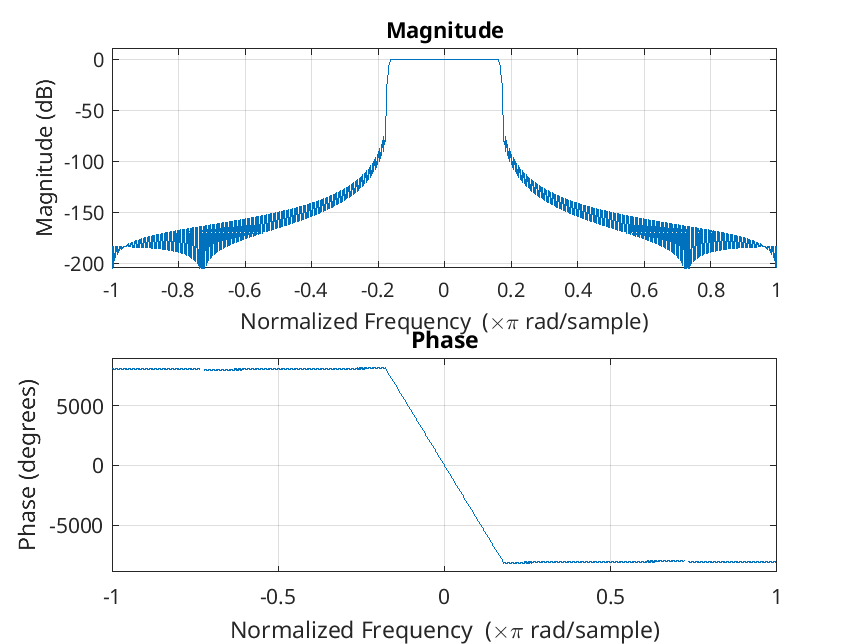
\includegraphics[width=10cm]{freqz_bl_512.png}
  \end{figure}

\section{Discussion: Samyak Sheersh}
\begin{enumerate}
  \item
\end{enumerate}
\end{document}
